%==============================================================================
% Chapitre 43 - Les poudres propulsives
%==============================================================================

\section{Introduction}

La poudre propulsive constitue la source principale d'énergie d'une
cartouche.

Sa combustion produit les gaz nécessaires à l'accélération du projectile
dans le canon.

Les poudres modernes représentent l'aboutissement de plusieurs siècles
d'évolution technologique.

\begin{aretenir}

La poudre propulsive transforme son énergie chimique en énergie mécanique
par l'intermédiaire des gaz produits lors de sa combustion.

\end{aretenir}

\section{Rôle de la poudre}

La poudre doit :

\begin{itemize}
    \item s'enflammer rapidement ;
    \item brûler de manière contrôlée ;
    \item produire une quantité importante de gaz ;
    \item générer une pression adaptée ;
    \item assurer une vitesse initiale régulière.
\end{itemize}

Son comportement influence directement les performances balistiques.

\section{Un point de vocabulaire}

Contrairement à une idée répandue, la poudre d'une cartouche moderne
n'explose généralement pas.

Elle brûle très rapidement.

On parle de combustion rapide ou de déflagration.

Cette distinction est fondamentale.

\begin{aretenir}

La poudre propulsive déflagre ; elle ne détonne pas.

\end{aretenir}

\begin{figure}[htbp]
\centering

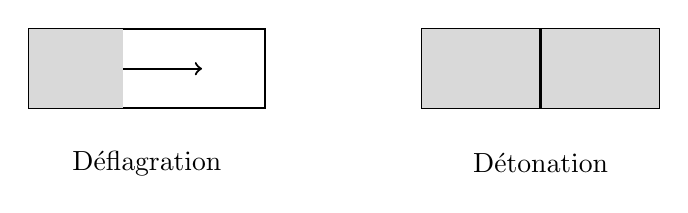
\begin{tikzpicture}[scale=1]

% Déflagration
\draw[thick] (0,0) rectangle (3,1);

\fill[gray!30] (0,0) rectangle (1.2,1);

\draw[->,thick] (1.2,0.5) -- (2.2,0.5);

\node at (1.5,-0.7) {Déflagration};

% Détonation
\draw[thick] (5,0) rectangle (8,1);

\fill[gray!30] (5,0) rectangle (8,1);

\draw[very thick] (6.5,0) -- (6.5,1);

\node at (6.5,-0.7) {Détonation};

\end{tikzpicture}

\caption{Illustration simplifiée d'une déflagration et d'une détonation.}
\label{fig:deflagration_detonation}
\end{figure}

\section{La poudre noire}

Pendant plusieurs siècles, les armes à feu ont utilisé la poudre noire.

Elle est traditionnellement constituée :

\begin{itemize}
    \item de nitrate de potassium ;
    \item de charbon ;
    \item de soufre.
\end{itemize}

Son utilisation a marqué l'histoire des armes à feu.

\section{Limites de la poudre noire}

La poudre noire présente plusieurs inconvénients :

\begin{itemize}
    \item production importante de fumée ;
    \item encrassement élevé ;
    \item rendement énergétique limité ;
    \item forte sensibilité à l'humidité.
\end{itemize}

Ces limitations ont conduit au développement de poudres plus performantes.

\section{Les poudres sans fumée}

La majorité des munitions modernes utilisent des poudres sans fumée.

Leur développement à la fin du XIX\ieme\ siècle a profondément transformé la
balistique.

Leurs avantages incluent :

\begin{itemize}
    \item une énergie plus élevée ;
    \item moins de résidus ;
    \item une meilleure régularité ;
    \item une réduction importante de la fumée.
\end{itemize}

\section{La nitrocellulose}

La nitrocellulose constitue le principal composant des poudres modernes.

Cette substance possède une forte capacité énergétique tout en restant
suffisamment stable pour être utilisée comme propulsif.

Elle est parfois appelée coton-poudre.

\section{Poudres simple base}

Les poudres dites simple base sont principalement constituées de
nitrocellulose.

Elles présentent généralement :

\begin{itemize}
    \item une bonne stabilité ;
    \item une combustion régulière ;
    \item une fabrication relativement simple.
\end{itemize}

\section{Poudres double base}

Les poudres double base contiennent généralement :

\begin{itemize}
    \item de la nitrocellulose ;
    \item de la nitroglycérine.
\end{itemize}

L'ajout de nitroglycérine augmente l'énergie disponible.

\section{Poudres triple base}

Certaines applications militaires utilisent des poudres triple base.

Celles-ci peuvent notamment contenir :

\begin{itemize}
    \item de la nitrocellulose ;
    \item de la nitroglycérine ;
    \item de la nitroguanidine.
\end{itemize}

Ces formulations sont principalement rencontrées dans les systèmes de gros
calibre.

\section{Formes des grains}

Les poudres propulsives existent sous différentes formes.

On rencontre notamment :

\begin{itemize}
    \item des grains sphériques ;
    \item des paillettes ;
    \item des bâtonnets ;
    \item des tubes perforés.
\end{itemize}

La géométrie influence fortement la combustion.

\begin{figure}[htbp]
\centering
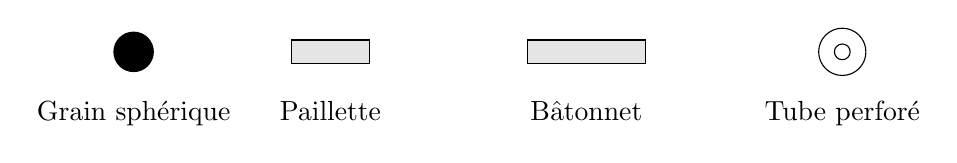
\begin{tikzpicture}[scale=1]

% Grain sphérique
\filldraw (0,0) circle (0.25);
\node[below] at (0,-0.5) {Grain sphérique};

% Paillette
\draw[fill=gray!20] (2,-0.15) rectangle (3,0.15);
\node[below] at (2.5,-0.5) {Paillette};

% Bâtonnet
\draw[fill=gray!20] (5,-0.15) rectangle (6.5,0.15);
\node[below] at (5.75,-0.5) {Bâtonnet};

% Tube perforé
\draw (9,0) circle (0.3);
\draw (9,0) circle (0.1);
\node[below] at (9,-0.5) {Tube perforé};

\end{tikzpicture}
\caption{Exemples de formes de grains utilisées dans les poudres propulsives.}
\label{fig:formes_grains}
\end{figure}

\section{Surface de combustion}

La vitesse de combustion dépend notamment de la surface exposée.

Lorsque la surface évolue pendant la combustion :

\begin{itemize}
    \item la production de gaz évolue ;
    \item la pression évolue ;
    \item les performances changent.
\end{itemize}

La forme des grains est donc un paramètre essentiel.

\begin{figure}[htbp]
\centering

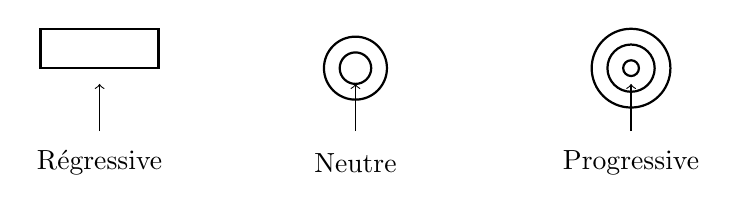
\begin{tikzpicture}[scale=1]

% Régressive
\draw[thick] (0,0) rectangle (1.5,0.5);
\draw[->] (0.75,-0.8) -- (0.75,-0.2);
\node at (0.75,-1.2) {Régressive};

% Neutre
\draw[thick] (4,0) circle (0.4);
\draw[thick] (4,0) circle (0.2);
\draw[->] (4,-0.8) -- (4,-0.2);
\node at (4,-1.2) {Neutre};

% Progressive
\draw[thick] (7.5,0) circle (0.5);
\draw[thick] (7.5,0) circle (0.3);
\draw[thick] (7.5,0) circle (0.1);
\draw[->] (7.5,-0.8) -- (7.5,-0.2);
\node at (7.5,-1.2) {Progressive};

\end{tikzpicture}

\caption{Influence de la géométrie des grains sur l'évolution de la surface de combustion.}
\label{fig:surface_combustion}
\end{figure}

\section{Combustion progressive}

Certaines poudres sont conçues pour présenter une combustion progressive.

Au cours de la combustion :

\begin{itemize}
    \item la surface disponible augmente ;
    \item la production de gaz reste importante ;
    \item l'accélération du projectile est prolongée.
\end{itemize}

Ces poudres sont particulièrement adaptées aux armes à canon long.

\section{Combustion régressive}

Dans d'autres cas :

\begin{itemize}
    \item la surface diminue progressivement ;
    \item la production de gaz décroît ;
    \item la pression chute plus rapidement.
\end{itemize}

\section{Vivacité}

La vivacité caractérise la rapidité de combustion d'une poudre.

Une poudre vive :

\begin{itemize}
    \item brûle rapidement ;
    \item produit rapidement sa pression maximale.
\end{itemize}

Une poudre lente :

\begin{itemize}
    \item brûle plus progressivement ;
    \item maintient la pression plus longtemps.
\end{itemize}

\section{Choix de la poudre}

Le choix d'une poudre dépend notamment :

\begin{itemize}
    \item du calibre ;
    \item de la masse du projectile ;
    \item de la longueur du canon ;
    \item des performances recherchées.
\end{itemize}

Une poudre inadaptée peut dégrader les performances ou provoquer des
surpressions dangereuses.

\begin{figure}[htbp]
\centering

\begin{tikzpicture}[scale=1]

\draw[->] (0,0) -- (8,0) node[right] {Temps};

\draw[->] (0,0) -- (0,5) node[above] {Pression};

% Poudre vive
\draw[thick]
(0,0)
.. controls (0.8,4.5) and (1.5,4) ..
(3,0);

\node at (1.8,4.2) {Poudre vive};

% Poudre lente
\draw[thick]
(0,0)
.. controls (2,2.5) and (4.5,3.5) ..
(7,0);

\node at (5.5,3.0) {Poudre lente};

\end{tikzpicture}

\caption{Évolution simplifiée de la pression pour une poudre vive et une poudre lente.}
\label{fig:vivacite_poudre}
\end{figure}

\section{Température}

La température influence le comportement des poudres.

Elle peut modifier :

\begin{itemize}
    \item la vitesse de combustion ;
    \item la pression maximale ;
    \item la vitesse initiale.
\end{itemize}

Certaines poudres sont spécialement formulées pour limiter cette sensibilité.

\section{Vieillissement}

Les poudres évoluent lentement au cours du temps.

Leur stabilité dépend notamment :

\begin{itemize}
    \item des conditions de stockage ;
    \item de la température ;
    \item de l'humidité ;
    \item de leur composition chimique.
\end{itemize}

\section{Sécurité}

Les poudres propulsives doivent être manipulées avec précaution.

Elles contiennent une quantité importante d'énergie chimique.

Le respect des procédures de stockage et de manipulation est essentiel.

\section{Vers la balistique intérieure}

La poudre constitue la source d'énergie du tir.

Cependant, ce n'est qu'au moment de sa combustion que cette énergie est
transformée en pression puis en mouvement.

Nous étudierons ce processus en détail dans la partie consacrée à la
balistique intérieure.

\section{À retenir}

\begin{aretenir}

\begin{itemize}
    \item La poudre propulsive constitue la source d'énergie du tir.
    \item Les poudres modernes sont principalement à base de
          nitrocellulose.
    \item La forme des grains influence la combustion.
    \item La vivacité caractérise la rapidité de combustion.
    \item La poudre déflagre et ne détonne pas.
\end{itemize}

\end{aretenir}
